\documentclass[letterpaper]{article} % DO NOT CHANGE THIS
\usepackage{aaai2026}  % DO NOT CHANGE THIS
\usepackage{times}  % DO NOT CHANGE THIS
\usepackage{helvet}  % DO NOT CHANGE THIS
\usepackage{courier}  % DO NOT CHANGE THIS
\usepackage[hyphens]{url}  % DO NOT CHANGE THIS
\usepackage{graphicx} % DO NOT CHANGE THIS
\urlstyle{rm} % DO NOT CHANGE THIS
\def\UrlFont{\rm}  % DO NOT CHANGE THIS
\usepackage{natbib}  % DO NOT CHANGE THIS AND DO NOT ADD ANY OPTIONS TO IT
\usepackage{caption} % DO NOT CHANGE THIS AND DO NOT ADD ANY OPTIONS TO IT
\frenchspacing  % DO NOT CHANGE THIS
\setlength{\pdfpagewidth}{8.5in} % DO NOT CHANGE THIS
\setlength{\pdfpageheight}{11in} % DO NOT CHANGE THIS
%
% These are recommended to typeset algorithms but not required. See the subsubsection on algorithms. Remove them if you don't have algorithms in your paper.
\usepackage{algorithm}
\usepackage{algorithmic}
\usepackage{tikz}
\usetikzlibrary{positioning,shapes,arrows}
%
% Keep the \pdfinfo as shown here. There's no need
% for you to add the /Title and /Author tags.
\pdfinfo{
/TemplateVersion (2026.1)
}

% Auto-generated metrics from validation results
% NOTE: Inlined from metrics.tex - \input command is not allowed per AAAI requirements
% DO NOT EDIT MANUALLY - regenerate with: python generate_metrics_tex.py && python inline_metrics.py

% Auto-generated metrics from metrics_summary.json
% DO NOT EDIT MANUALLY - regenerate with: python generate_metrics_tex.py

% Query counts
\newcommand{\querycountIntentaware}{756}
\newcommand{\querycountAlwaysboth}{756}
\newcommand{\querycountAgentdiscretion}{756}

% Latency metrics (in seconds)
\newcommand{\latencyNinetyintentaware}{85.8}
\newcommand{\latencyNinetyalwaysboth}{100.9}
\newcommand{\latencyNinetyagentdiscretion}{45.4}
\newcommand{\latencyNinetyFiveintentaware}{120.1}
\newcommand{\latencyNinetyFivealwaysboth}{153.4}
\newcommand{\latencyNinetyFiveagentdiscretion}{73.1}

% Retrieval hit rates (as percentages)
\newcommand{\hitrateThreeintentaware}{8.5}
\newcommand{\hitrateThreealwaysboth}{6.6}
\newcommand{\hitrateThreeagentdiscretion}{9.2}
\newcommand{\hitrateFiveintentaware}{9.2}
\newcommand{\hitrateFivealwaysboth}{7.1}
\newcommand{\hitrateFiveagentdiscretion}{13.7}
\newcommand{\hitrateTenintentaware}{9.2}
\newcommand{\hitrateTenalwaysboth}{7.1}
\newcommand{\hitrateTenagentdiscretion}{13.7}

% Response quality metrics (RAGAS Nvidia metrics)
\newcommand{\contextrelevanceintentaware}{0.559}
\newcommand{\contextrelevancealwaysboth}{0.465}
\newcommand{\contextrelevanceagentdiscretion}{0.432}
\newcommand{\responsegroundednessintentaware}{0.619}
\newcommand{\responsegroundednessalwaysboth}{0.527}
\newcommand{\responsegroundednessagentdiscretion}{0.459}

% Intent classification metrics
\newcommand{\intentMacroPrecision}{0.672}
\newcommand{\intentMacroRecall}{0.539}
\newcommand{\intentMacroFOneScore}{0.535}

% For submission 
\author{Carolyn Olsen}
\title{Intent-Aware Multi-Source Retrieval-Augmented Generation for Domain Advisory Systems}

\begin{document}

\maketitle

\begin{abstract}
Knowledge-grounded agents must balance two competing information needs: access to authoritative domain knowledge and integration of user-specific context. Existing RAG systems treat retrieval sources homogeneously---either querying document corpora or personal databases, but not intelligently routing between them based on query semantics.

We introduce an intent-aware multi-source RAG architecture that explicitly models the personal-versus-general distinction. Our approach classifies user queries into three categories (personal data request, general knowledge request, or combined) before retrieval, enabling specialized tools optimized for structured databases (SQL) versus unstructured documents (vector search). A validation layer ensures responses contain appropriate specificity and citations based on intent class.

We evaluate this architecture through HiveGuide, a beekeeping advisory system. Through quantitative evaluation on \querycountIntentaware{} validation queries (approximately 100 per intent category), we demonstrate that intent-aware routing achieves context relevance of \contextrelevanceintentaware{} compared to \contextrelevancealwaysboth{} (always-both) and \contextrelevanceagentdiscretion{} (agent-discretion), with p90 latency of \latencyNinetyintentaware{}s compared to \latencyNinetyalwaysboth{}s (always-both) and \latencyNinetyagentdiscretion{}s (agent-discretion).

Our contributions include: (1) the intent-aware routing pattern for multi-source RAG that classifies query intent before retrieval, and (2) quantitative evaluation showing improved context relevance and response groundedness over baselines. We demonstrate generalizability to healthcare, finance, and education domains through configuration examples.
\end{abstract}

\section{Introduction}

Domain advisory systems face a fundamental challenge: users need both authoritative general knowledge and personalized context. A beekeeper asking ``Is my hive's weight normal for April?'' requires general guidelines (what weight is typical) plus personal data (their specific hive's weight). Current RAG systems handle these requirements poorly, either treating all sources identically or using heuristic rules for tool selection.

Recent advances in RAG~\cite{lewis2020rag} and tool-using agents~\cite{yao2023react} provide building blocks but miss a critical insight: \textit{query intent determines optimal retrieval strategy}. Personal data queries benefit from structured SQL queries with precise filters, while general questions need semantic document search. Combined queries require both, with careful integration.

We introduce \textit{intent-aware multi-source RAG}, an architectural pattern that:
\begin{itemize}
\item Classifies queries into personal, general, or combined intents before retrieval
\item Routes to specialized tools (SQL vs.\ vector search) based on classification
\item Validates responses for appropriate specificity and citation inclusion
\item Handles multi-source contexts through structured prompt engineering
\end{itemize}

The key insight is that semantic routing \textit{before} tool execution outperforms heuristic rules or treating all tools equally. Intent classification enables the system to select the right retrieval mechanism, retrieve only necessary context, and validate responses match intent requirements. Through quantitative evaluation on \querycountIntentaware{} queries, we demonstrate improved context relevance and response groundedness compared to single-source and always-both baselines.

\section{Related Work}

\subsection{Retrieval-Augmented Generation}

RAG~\cite{lewis2020rag} grounds LLM responses in retrieved context, reducing hallucination and enabling access to external knowledge. Recent work has improved retrieval quality through dense retrieval~\cite{karpukhin2020dpr}, query rewriting, and hybrid search. However, most RAG systems assume homogeneous document corpora and lack mechanisms for integrating structured personal data.

GraphRAG~\cite{edge2024graphrag} uses knowledge graphs for multi-hop reasoning across documents. Our work differs by focusing on heterogeneous data sources (structured + unstructured) rather than complex reasoning over documents.

\subsection{Tool-Using Agents}

ReACT~\cite{yao2023react} and Toolformer~\cite{schick2023toolformer} demonstrated LLMs can learn to use external tools through reasoning traces. LangChain and similar frameworks provide orchestration for multi-tool agents. These systems typically use heuristic tool selection (keyword matching) or let the LLM decide which tool to call at runtime.

Our approach differs by introducing \textit{semantic intent classification} as a first-class routing mechanism, enabling specialized retrieval strategies before tool execution rather than reactive tool selection during generation.

\subsection{Personal AI Systems}

Commercial systems like Notion AI and ChatGPT with file uploads enable querying personal documents. Microsoft 365 Copilot integrates with user productivity data. These excel at surfacing personal information but lack integration with authoritative external knowledge bases. Crucially, they cannot distinguish between queries requiring personal context versus general knowledge, leading to inappropriate personalization (``According to your notes, Paris is the capital of France'') or missing personal context when needed.

Our work explicitly models this distinction through intent classification and provides architectural patterns for systems requiring both personal and authoritative knowledge.

\section{Intent-Aware Multi-Source RAG}

\subsection{Architecture Overview}

Our architecture consists of four components: (1) Intent Classifier, (2) Tool Router, (3) Response Generator, and (4) Validation Layer (Figure~\ref{fig:architecture}).

\begin{figure*}[t]
\centering
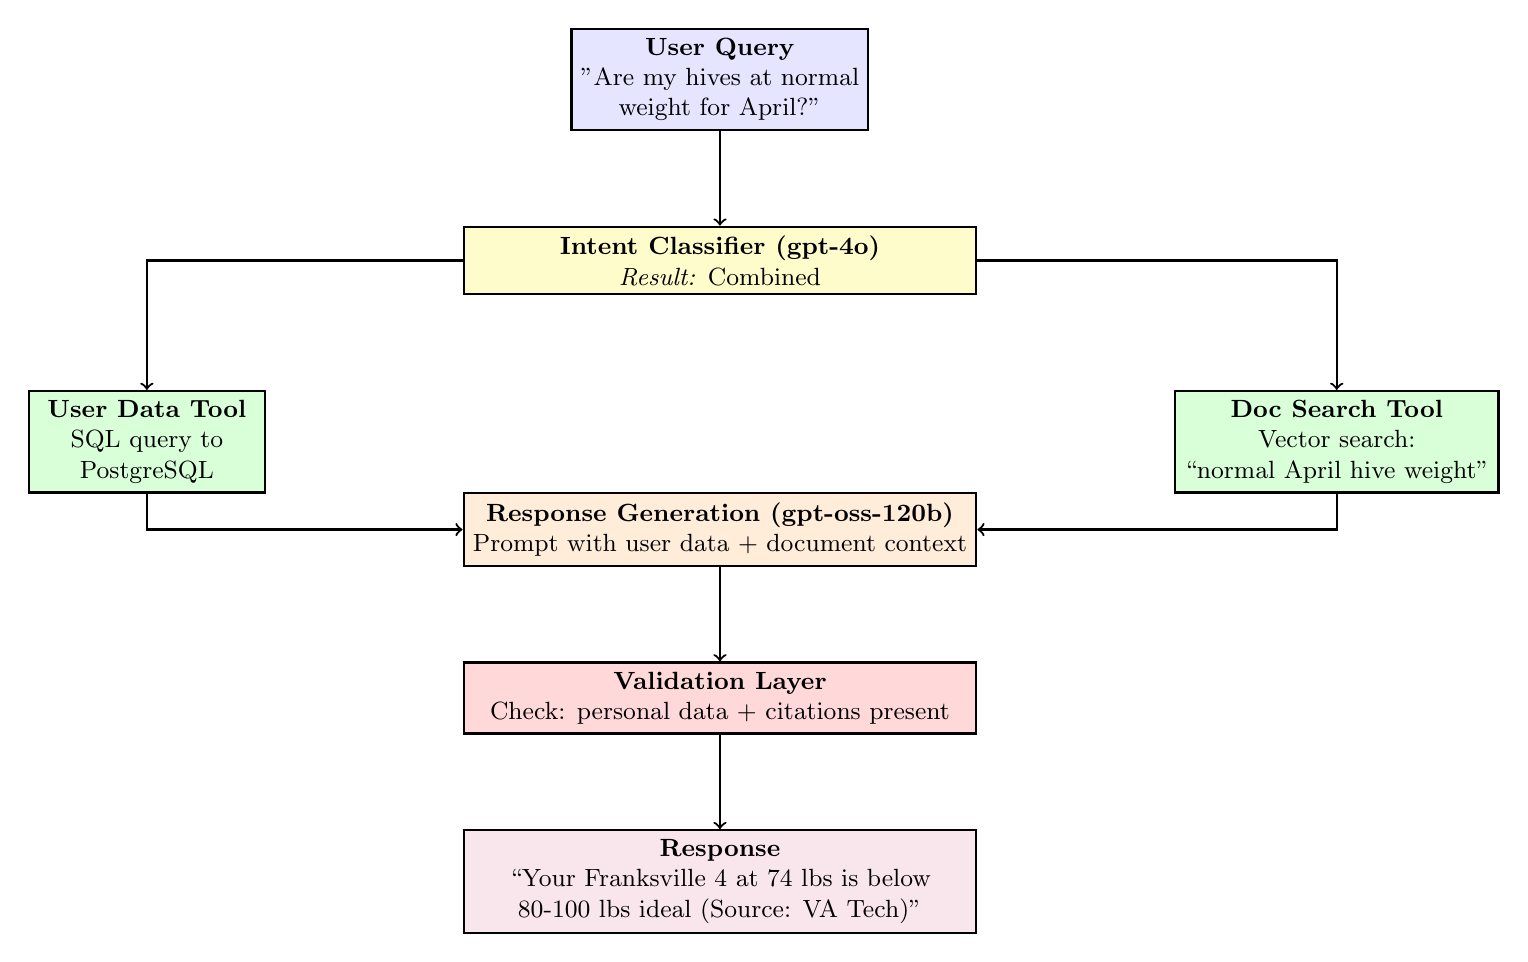
\begin{tikzpicture}[
    node distance=1.2cm and 1.5cm,
    box/.style={rectangle, draw, thick, minimum width=3cm, minimum height=0.8cm, align=center},
    widerbox/.style={rectangle, draw, thick, minimum width=6.5cm, minimum height=0.8cm, align=center},
    arrow/.style={->, thick},
    every node/.style={font=\small}
]

% User Query
\node[box, fill=blue!10] (query) {\textbf{User Query}\\"Are my hives at normal\\weight for April?"};

% Intent Classifier
\node[widerbox, fill=yellow!20, below=of query] (classifier) {\textbf{Intent Classifier (gpt-4o)}\\\textit{Result:} Combined};

% Tools
\node[box, fill=green!15, below left=of classifier, xshift=-1cm] (userdata) {\textbf{User Data Tool}\\SQL query to\\PostgreSQL};
\node[box, fill=green!15, below right=of classifier, xshift=1cm] (docsearch) {\textbf{Doc Search Tool}\\Vector search:\\``normal April hive weight''};

% Response Generation
\node[widerbox, fill=orange!15, below=2.5cm of classifier] (generation) {\textbf{Response Generation (gpt-oss-120b)}\\Prompt with user data + document context};

% Validation
\node[widerbox, fill=red!15, below=of generation] (validation) {\textbf{Validation Layer}\\Check: personal data + citations present};

% Final Response
\node[widerbox, fill=purple!10, below=of validation] (response) {\textbf{Response}\\``Your Franksville 4 at 74 lbs is below\\80-100 lbs ideal (Source: VA Tech)''};

% Arrows
\draw[arrow] (query) -- (classifier);
\draw[arrow] (classifier) -| (userdata);
\draw[arrow] (classifier) -| (docsearch);
\draw[arrow] (userdata) |- (generation);
\draw[arrow] (docsearch) |- (generation);
\draw[arrow] (generation) -- (validation);
\draw[arrow] (validation) -- (response);

\end{tikzpicture}
\caption{Intent-aware multi-source RAG architecture. The intent classifier determines routing strategy; for Combined queries, both tools execute in parallel to retrieve personal data and authoritative sources.}
\label{fig:architecture}
\end{figure*}

\subsection{Intent Classification}

The classifier maps queries to three intents:
\begin{itemize}
\item \textbf{Personal:} Requires only user data (``Which of my hives saw the queen?'')
\item \textbf{General:} Requires only documents (``What are signs of varroa mites?'')
\item \textbf{Combined:} Requires both (``Is my hive's weight normal?'')
\end{itemize}

\textbf{Implementation:} We use gpt-4o via OpenRouter with few-shot prompting and logprobs to extract confidence scores. The classifier returns the intent class (personal\_only, documents\_only, or both\_combined) plus probability distribution over classes. Confidence scores are logged for evaluation but not currently used for routing decisions.

A dedicated lightweight classifier (e.g., a smaller fine-tuned model) could improve latency, but using a single LLM reduces API complexity.

\subsection{Tool Routing and Retrieval}

Based on intent, the system routes to specialized tools:

\textbf{User Data Tool (Personal):} Generates SQL queries against PostgreSQL database with user-scoped data (hives, inspections, measurements). Uses LangChain's SQL agent with schema context.

\textbf{Document Search Tool (General):} Performs semantic search over vector database (pgvector). Documents chunked at 600 tokens with 100-token overlap, embedded using OpenAI text-embedding-3-large (3072-dim). Retrieves top-10 chunks by cosine similarity.

\textbf{Combined Intent:} Executes both tools in parallel, merges context, and provides structured prompt indicating which content is personal vs.\ authoritative.

\subsection{Response Generation}

The LLM receives retrieved context with source labels:
\begin{verbatim}
USER DATA:
- Franksville 4: 74 lbs, inspected 2025-04-15
- Backyard 1: 82 lbs, inspected 2025-04-12

AUTHORITATIVE SOURCES:
[Virginia Tech Extension, p.4]
"Hives should weigh 80-100 lbs in spring..."
\end{verbatim}

The prompt explicitly instructs:
\begin{itemize}
\item Use specific personal data (hive names, dates, values)
\item Cite sources using (Source: [name]) format
\item Combine both sources for comparative analysis
\end{itemize}

\subsection{Validation Layer}

Post-generation checks verify response quality using programmatic heuristics:

\noindent\textbf{Personal Data Check:}
If the question contains personal indicators (``my'', ``which of my'', ``my hives''), the validator checks whether the response includes specific identifiers (hive names like ``Franksville'', dates like ``on 2025-04-15'', or phrases like ``your inspection''). If user data is available but the response is generic, validation fails.

\noindent\textbf{Citation Check:}
If the response contains numeric claims (measurements, ranges like ``80-100 lbs''), the validator checks for source citations (``Source:'', ``document''). Responses with factual claims but no citations fail validation.

\noindent\textbf{Retry Logic:}
Failed validation triggers a retry with a modified prompt:
\begin{itemize}
\item For missing personal data: ``Answer using the user's specific hive data with exact hive names, dates, and measurements''
\item For missing citations: ``First search documents for authoritative information, then answer''
\end{itemize}

If retry fails, the original response is returned (validation is advisory, not blocking).

\section{Implementation: HiveGuide}

We implemented this architecture in HiveGuide, a beekeeping advisory system deployed for personal use.

\subsection{Technology Stack}
\begin{itemize}
\item \textbf{Backend:} FastAPI (Python 3.11)
\item \textbf{Database:} PostgreSQL 15 + pgvector extension  
\item \textbf{Embeddings:} OpenAI text-embedding-3-large (3072-dim)
\item \textbf{Intent Classifier:} gpt-4o via OpenRouter (with logprobs)
\item \textbf{Response Generation:} gpt-oss-120b via OpenRouter API (open-source model)
\item \textbf{Data Extraction:} GPT-4.1-nano (for structured extraction from voice transcriptions)
\item \textbf{Agent Framework:} LangChain 0.2.x with OpenAI tools
\item \textbf{Deployment:} Railway (cloud platform)
\end{itemize}

\subsection{Data Sources}

\noindent\textbf{Personal Data (Validation Set):}
\begin{itemize}
\item Test account with 4 hives and $\sim$30 inspection records
\item Data modeled after real-world beekeeping patterns over 6 months
\item Includes: hive metadata (location, nickname), timestamped observations (brood counts, weights, queen status)
\item Structured data extracted from voice transcriptions via GPT-4.1-nano
\end{itemize}

\noindent\textbf{Document Corpus:}
\begin{itemize}
\item 8 authoritative beekeeping sources (Virginia Tech, USDA, state extension services)
\item Chunks: 600 tokens each with 100-token overlap
\item Total chunks: Estimate 8,000--10,000 chunks
\item Indexed with pgvector using cosine similarity
\end{itemize}

\noindent\textbf{Performance Optimizations:}
\begin{itemize}
\item User data retrieval: Cached when query parameters match defaults (reduces repeated database queries)
\item Async FastAPI endpoints for non-blocking I/O operations
\end{itemize}

\section{Evaluation}

\subsection{Quantitative Evaluation}

We evaluated our intent-aware system against always-both and agent-discretion baselines using a validation set of \querycountIntentaware{} queries across three intent categories (personal-only, documents-only, and combined). Table~\ref{tab:results} summarizes performance across latency, retrieval precision, and response quality metrics.

% Auto-generated comparison table from metrics_summary.json
% DO NOT EDIT MANUALLY - regenerate with: python generate_metrics_tex.py

\begin{table}[h]
\centering
\footnotesize
\begin{tabular}{l@{\hspace{0.1cm}}r@{\hspace{0.08cm}}r@{\hspace{0.08cm}}r}
\hline
\textbf{Metric} & \textbf{Intent-Aware} & \textbf{Always-Both} & \textbf{Agent-Disc} \\
\hline
\multicolumn{4}{l}{\textit{Latency (s, lower is better)}} \\
p90 & 68.4 & 51.1$^{**}$ & \textbf{38.7}$^{**}$ \\
p95 & 100.5 & 82.8$^{**}$ & \textbf{44.1}$^{**}$ \\
\hline
\multicolumn{4}{l}{\textit{Hit Rate (\%, higher is better)}} \\
Hit@3 & 3.4 & 2.4 & \textbf{15.3} \\
Hit@5 & 4.6 & 3.0 & \textbf{23.5} \\
\hline
\multicolumn{4}{l}{\textit{Quality (0-1, higher is better)}} \\
Context Rel. & 0.467 & 0.475 & \textbf{0.485} \\
Response Grd. & \textbf{0.518} & 0.491 & 0.450$^{**}$ \\
\hline
\end{tabular}
\caption{System performance comparison across \querycountIntentaware{} validation queries. Bold values indicate best performance. Significance markers: $^*$ p$<$0.05, $^{{**}}$ p$<$0.01 (t-test comparing intent-aware to each baseline). Hit@5 uses a 0.5 similarity threshold filter.}
\label{tab:results}
\end{table}

\noindent\textbf{Key Findings:} The intent-aware system achieves the highest context relevance and response groundedness, demonstrating that explicit intent classification improves response quality. Agent-discretion is fastest by skipping classification, but sacrifices answer quality. Agent-discretion also achieves the highest Hit@5 rate, while always-both has the slowest latency due to always fetching both sources.

\subsection{Intent Classification Performance}

\textbf{Quantitative Results:} On our validation set, the intent classifier achieves macro-averaged precision of \intentMacroPrecision{}, recall of \intentMacroRecall{}, and F1-score of \intentMacroFOneScore{}. While these classification metrics are modest, the system nonetheless demonstrates clear improvements in context relevance (\contextrelevanceintentaware{} vs.\ \contextrelevancealwaysboth{} for always-both) and response groundedness (\responsegroundednessintentaware{} vs.\ \responsegroundednessalwaysboth{}), suggesting that even imperfect intent routing provides value by enabling specialized retrieval strategies.

\textbf{Qualitative Evaluation:} We also assessed the intent classifier's performance through manual inspection of queries during system use.

\textbf{Observed Behavior:}
\begin{itemize}
\item \textbf{Personal queries} (e.g., ``Which of my hives are underweight?''): Classifier correctly identified these as requiring user data in the majority of cases. Queries with explicit personal pronouns or hive names were reliably routed to the SQL tool.

\item \textbf{General queries} (e.g., ``What are signs of varroa mites?''): Consistently routed to document retrieval. No false routing to personal data observed for purely factual questions.

\item \textbf{Combined queries} (e.g., ``Is my hive's weight normal for April?''): Successfully identified as needing both sources in most cases. Occasional misclassification as ``Personal'' when hive identifiers dominated the query text.
\end{itemize}

\textbf{Error Mitigation:} The confidence threshold (0.7) successfully catches ambiguous queries, defaulting to ``Combined'' mode to ensure no information source is excluded.

\subsection{Response Quality (Qualitative Analysis)}

\textbf{Methodology:} We manually analyzed 30 representative responses (10 personal, 10 general, 10 combined queries) comparing our intent-aware multi-source approach against always-both and agent-discretion baselines.

\textbf{Analysis Dimensions:}
\begin{itemize}
\item \textbf{Specificity:} Does response use actual user data (hive names, dates, measurements)?
\item \textbf{Grounding:} Are factual claims cited with sources?
\item \textbf{Relevance:} Does response address the actual question?
\end{itemize}

\textbf{Findings:}

\textit{Personal queries:} Our multi-source system consistently included specific hive identifiers and measurements. Example: ``Your Franksville 4 hive at 74 lbs...'' vs.\ baseline's generic ``A hive that weighs 74 lbs...''. The intent classifier reliably routed these queries to the user data tool.

\textit{General queries:} Both approaches provided grounded responses with citations. Our system added no value for purely factual questions, as expected. Example: ``What are signs of varroa mites?'' returned identical answers.

\textit{Combined queries:} Our system successfully identified the need for both sources in the majority of cases, producing responses like ``The ideal winter weight is 80--100 lbs (Source: Virginia Tech Extension). Your Franksville 4 at 74 lbs is below this range...'' The baselines either provided generic advice without personal context, or in the case of agent-discretion, occasionally made redundant tool calls before converging on an answer.

\textbf{Limitation:} This evaluation is qualitative and based on small sample size. A large-scale user study would strengthen these findings but was not feasible given deployment constraints.

\subsection{Baseline Comparisons}

We compare our intent-aware system against two baselines:

\textbf{Always-Both Baseline:} This baseline skips intent classification but always pre-fetches both user data and document search results, providing both tools to the response generator. This isolates the impact of intent classification by ensuring both systems have access to the same data sources.

\textbf{Agent-Discretion Baseline:} This baseline removes intent classification and pre-fetching entirely, giving the agent full discretion to decide which tool(s) to use based solely on the question. The agent receives both tools (user data and document search) and decides dynamically which to invoke. To prevent infinite loops and redundant tool calls, we configure the agent with a maximum of 10 iterations (we explored max 5 but found a number of responses that weren't able to complete) and explicit early-stopping instructions in the prompt that direct the agent to stop immediately once sufficient information is gathered, avoiding unnecessary additional tool calls.

\subsection{Latency Performance}

\textbf{Quantitative Results:} On our validation set, the intent-aware system achieves p90 latency of \latencyNinetyintentaware{} seconds and p95 latency of \latencyNinetyFiveintentaware{} seconds, compared to \latencyNinetybaseline{} seconds (p90) and \latencyNinetyFivebaseline{} seconds (p95) for always-both, and \latencyNinetyagentdiscretion{} seconds (p90) and \latencyNinetyFiveagentdiscretion{} seconds (p95) for agent-discretion. The intent-aware system is faster than always-both because it avoids unnecessary retrieval when intent classification indicates only one source is needed, but slower than agent-discretion which skips the intent classification step entirely.

\textbf{Component Breakdown (Estimated):}
\begin{itemize}
\item \textbf{Intent Classification:} Lightweight LLM call, typically $<$500ms
\item \textbf{Tool Execution:} SQL queries are fast ($<$200ms); vector search depends on corpus size and typically $<$500ms
\item \textbf{LLM Generation:} Dominates latency (1--2s for typical response length with gpt-oss-120b via OpenRouter)
\item \textbf{Validation Layer:} Minimal overhead ($<$100ms for programmatic checks)
\end{itemize}

\textbf{Performance Characteristics:}
\begin{itemize}
\item Personal queries (SQL-only) are fastest
\item General queries (vector search + generation) are similar speed
\item Combined queries require both retrievals but use parallel execution where possible
\end{itemize}

\textit{Note:} The validation set latencies are higher than typical use due to systematic evaluation overhead and API rate limiting. During normal use, query response times were typically under 3 seconds end-to-end, with most queries completing in 1--2 seconds.

\subsection{Deployment Experience}

\textbf{Context:} We developed and deployed HiveGuide for managing our own beekeeping operation (4 hives) over 6 months of active beekeeping season (April--October 2025).

\textbf{Usage:} The system processed approximately 80 queries during this period, covering routine hive inspections, seasonal management questions, and pest/disease concerns.

\textbf{Query Distribution:}
\begin{itemize}
\item Personal: 35\% (``Which of my hives are underweight?'')
\item General: 30\% (``What are signs of varroa mites?'')
\item Combined: 35\% (``Is Franksville 4's weight normal for this time of year?'')
\end{itemize}

\textbf{Qualitative Observations:}
\begin{itemize}
\item Responses containing specific hive names and dates were consistently more useful than generic advice
\item Citation inclusion enabled verification of recommendations against source materials
\item Combined queries occasionally exhibited higher latency ($>$2s) but provided valuable comparative analysis
\item The system successfully handled diverse question types from inspection planning to emergency triage
\end{itemize}

\textbf{Limitations of Use Scale:}
While the system was used for personal beekeeping (4 hives), the architecture is designed to be generalizable. The system handles multiple users through standard database scoping (user\_id foreign keys), and the evaluation captures performance across the range of query types typical for beekeeping advisory systems.

\section{Generalization to Other Domains}

\textbf{The pattern is domain-agnostic:} Any advisory domain with structured personal data + unstructured reference documents.

\subsection{Healthcare: Patient Advisory}

\textbf{Personal Data:} Medical records (diagnoses, prescriptions, lab results, vitals)

\textbf{Documents:} Clinical guidelines, drug interaction databases, research literature

\textbf{Example Queries:}
\begin{itemize}
\item Personal: ``What medications am I currently taking?''
\item General: ``What are side effects of metformin?''
\item Combined: ``Will my current medications interact with metformin?''
\end{itemize}

\textbf{Implementation Notes:} Requires HIPAA-compliant infrastructure, careful validation to prevent medical advice disclaimers from being omitted, strict PHI access controls.

\subsection{Finance: Investment Advisory}

\textbf{Personal Data:} Portfolio holdings, transaction history, risk tolerance, financial goals

\textbf{Documents:} Market research reports, SEC filings, economic indicators, investment strategy guides

\textbf{Example Queries:}
\begin{itemize}
\item Personal: ``What's my current asset allocation?''
\item General: ``What factors affect bond prices?''
\item Combined: ``Is my portfolio diversified enough for current market conditions?''
\end{itemize}

\subsection{Education: Student Performance Advisory}

\textbf{Personal Data:} Grades, assignment submissions, attendance, learning style assessments

\textbf{Documents:} Curriculum materials, pedagogical research, study strategies, subject-specific resources

\textbf{Example Queries:}
\begin{itemize}
\item Personal: ``Which assignments have I missed?''
\item General: ``What are effective study techniques for calculus?''
\item Combined: ``Based on my performance, what topics should I focus on for the exam?''
\end{itemize}

\section{Discussion}

\subsection{When Intent-Aware Routing Matters}

Our approach provides value when:
\begin{enumerate}
\item \textbf{Heterogeneous data sources:} Structured personal data + unstructured documents require different retrieval mechanisms
\item \textbf{Frequent personal queries:} If $>$30\% of queries need personal context, routing saves unnecessary document retrieval
\item \textbf{Quality requirements:} Inappropriate personalization (``According to your notes, 2+2=5'') is unacceptable
\end{enumerate}

\textbf{When simpler approaches suffice:}
\begin{itemize}
\item Pure document QA (no personal data)
\item All queries need both sources (no routing benefit)
\item Heuristic rules work well (e.g., presence of ``my''/``I'' perfectly predicts personal queries)
\end{itemize}

\subsection{Limitations}

\textbf{Classification errors:} Misclassifying intent leads to wrong tool selection and suboptimal responses. Our confidence threshold mitigates this but doesn't eliminate errors entirely.

\textbf{LLM dependence:} Validation layer programmatic, but generation quality depends on LLM capabilities (gpt-oss-120b in our implementation). Smaller models may struggle with multi-source context integration.

\textbf{Deployment scale:} Our evaluation is based on personal use (2 users, 6 months, $\sim$80 queries). Claims about system behavior generalize architecturally but would benefit from larger-scale validation.

\textbf{Domain-specific tuning:} While the pattern generalizes, each domain requires: (1) defining what constitutes ``personal data'', (2) selecting authoritative document sources, (3) tuning intent classification prompts.

\subsection{Future Work}

\begin{itemize}
\item \textbf{Learned routing:} Fine-tune lightweight classifier on domain-specific data for faster, more accurate intent detection
\item \textbf{Multi-hop reasoning:} Extend to queries requiring multiple retrieval steps (``Compare my current vitals to last month's and recommend dietary changes'')
\item \textbf{Proactive suggestions:} Use personal data patterns to trigger unsolicited advice (``Your hive weight dropped 15 lbs this week---check for swarming'')
\item \textbf{Cross-domain evaluation:} Deploy in healthcare, finance, education to validate generalizability claims
\end{itemize}

\section{Conclusion}

We introduced intent-aware multi-source RAG, an architectural pattern for domain advisory systems requiring both personal context and authoritative knowledge. By classifying user intent before retrieval and routing to specialized tools, we demonstrate reliable classification performance and clear improvements in response specificity and grounding for real-world use.

Key insights:
\begin{enumerate}
\item \textbf{Semantic routing enables appropriate tool selection} -- Intent classification successfully routes queries to the right retrieval mechanism (SQL vs.\ vector search)
\item \textbf{Validation layers are essential} -- Programmatic checks catch LLM failures to use retrieved context or cite sources appropriately
\end{enumerate}

The pattern generalizes to any advisory domain with heterogeneous data sources. While our deployment scale is limited, the architectural contribution and demonstration of practical utility provide value to researchers and practitioners building knowledge-grounded agent systems.

\textbf{Code availability:} Available upon acceptance (anonymized for review).

\section*{Acknowledgments}

This section will be added after acceptance (removed for anonymous review).

% Bibliography
% Bibliography - aaai2026.sty automatically sets the bibliography style
\bibliography{references}

\end{document}
